\documentclass[11pt, a4paper]{article}
\usepackage[letterpaper, portrait, margin=0.5in]{geometry}
\usepackage[english]{babel}  % force American English hyphenation patterns
\usepackage{amsmath,mathtools}

\usepackage{graphicx}
\usepackage{wrapfig}


\begin{document}
\title{Chapter 22 Gauss's Law}
\author{Apostolos Delis}
\date{\today}
\maketitle

\tableofcontents
\section[22.1 Charge and Electric flux]{Charge and Electric flux}
\begin{itemize}
    \item Gauss's Law fundamentally, is, given a general distribution of charge, we can
        surround it with an imaginary surface that encloses the charge.
    \item  Gauss's law is a relationship between the field at all the points on the
        surface and the total charge enclosed within the surface.
    \item When you have the imaginary surface, you can move a test charge $q_0$ around
        the vicinity of the surface.
    \item By measuring the force $\vec{\mathbf{f}}$ experienced by the test charge, you
        make a three dimensional map of the electric field
        $\vec{\mathbf{E}} = \frac{\vec{\mathbf{f}}}{q_0}$
\end{itemize}
\subsection{Electric flux and Enclosed Charge}
\begin{itemize}
    \item  the electric-field vectors point out of the surface, we say that there is an
        outward electric flux
    \item This can be thought of similar to how fluid moves and has flux within regions,
        even though electric fields don't technically move, they can be thought of as
        a flow
    \item The following images show a simple relationship. Positive charge inside the
        box goes with an outward electric flux through the box's surface, and negative
        charge inside goes with an inward electric flux.

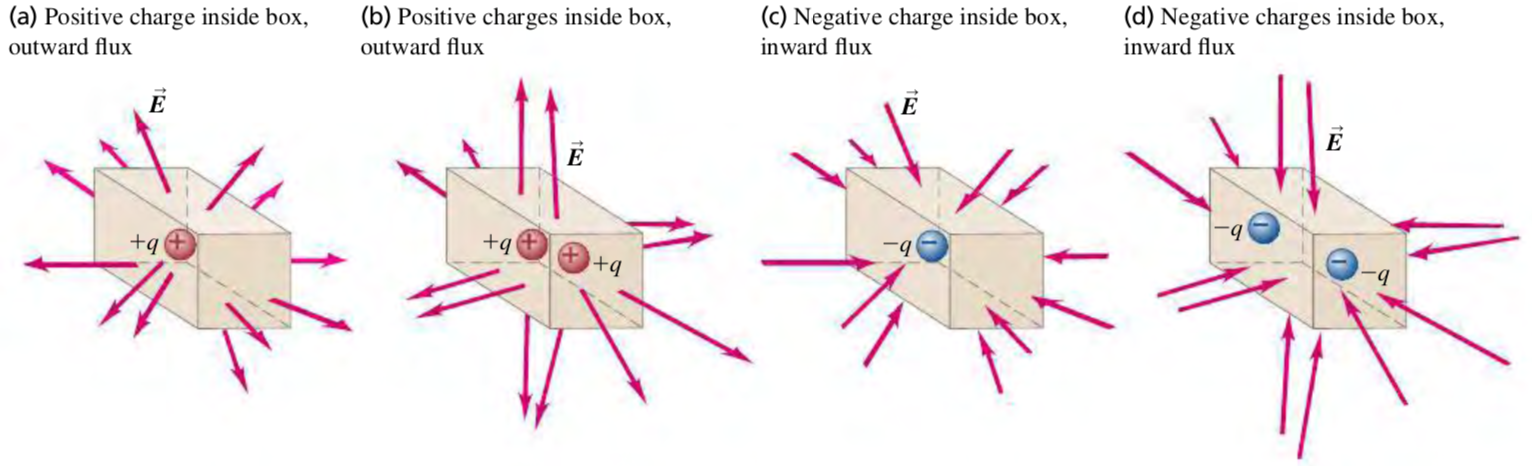
\includegraphics[scale=0.65]{images/electric_flux.png}

    \item If the positive and negative charges cancel each other out, then the amount of
        charge entering or leaving the system is 0, so the flux is zero
    \item The magnitude of the electric flux decreases with distance to $\frac{1}{r^2}$
\end{itemize}

\section[22.2, Calculating Electric flux]{Calculating Electric flux}
The net electric flux through a closed surface is directly proportional to the net charge
inside that surface. To calculate this, use the analogy of the field of velocity vectors
$\vec{\mathbf{v}}$ and the electric field $\vec{\mathbf{E}}$
\subsection{flux of a Uniform Electric field}
\begin{itemize}
    \item We define the electric flux through this area to be the product of the field
        magnitude $E$ and the area $A$
        \begin{equation}
            \Phi_E = EA
        \end{equation}
    \item flux can be thought of as the number of lines passing through $A$, so the more
        lines passing through $A$, the larger the magnitude of $\Phi_E$
    \item The electric flux $\Phi_E$ through the surface equals the scalar product of the
        electric field $\vec{\mathbf{E}}$ and the area vector $\vec{\mathbf{A}}$

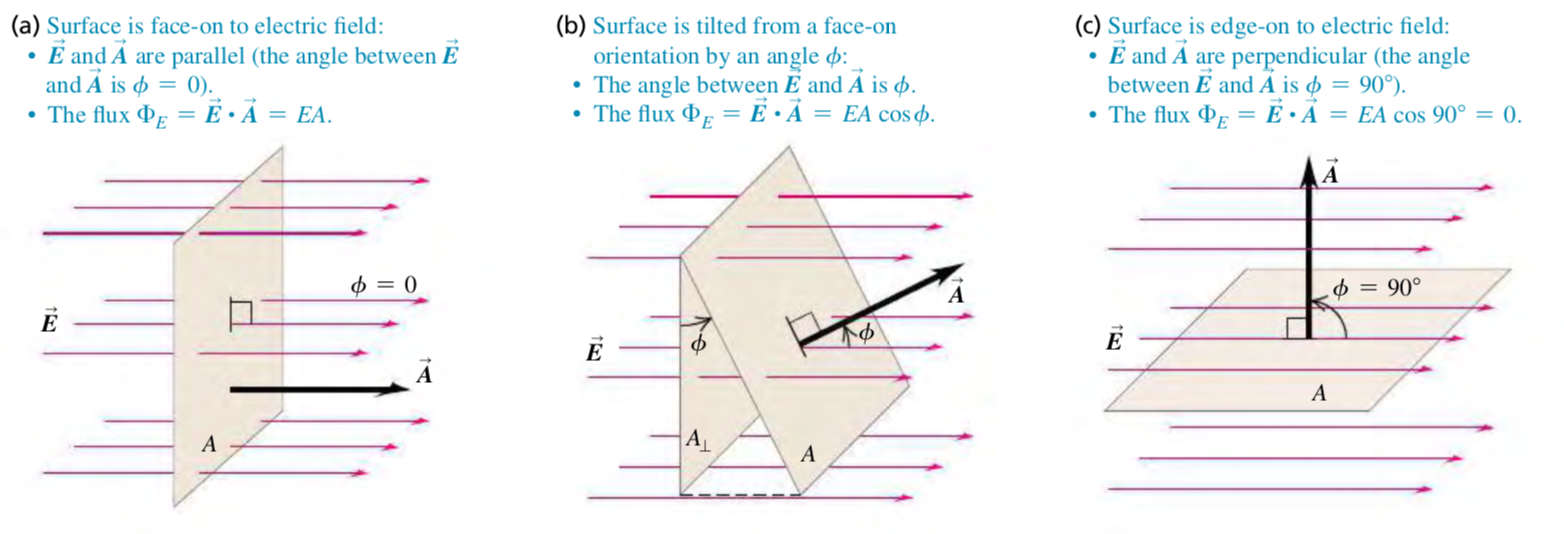
\includegraphics[scale=0.65]{images/flat_surface_flux.png}

    \item When $A$ is flat, but not perpendicular to the field $\vec{\mathbf{E}}$, then
        fewer field lines pass through it. The area that counts is the area $A_{\perp}$
        and is equal to
        \begin{equation}
            \Phi_E = EA\cos\phi
        \end{equation}
    \item Since $E\cos\phi$ is a component of $\vec{\mathbf{E}}$, we can rewrite this as:
        \begin{equation}
            \Phi_E = E_{\perp}A
        \end{equation}
    \item In terms of the vector area $\vec{\mathbf{A}}$, we can write the electric flux
        as the scalar product of $\vec{\mathbf{E}}$ and $\vec{\mathbf{A}}$
        \begin{equation}
            \Phi_E = \vec{\mathbf{E}} \cdot \vec{\mathbf{A}}
        \end{equation}
    \item We can represent the direction of the vector area $\vec{\mathbf{A}}$ by using
        the unit vector $\hat{\mathbf{n}}$, then:
        \begin{equation}
            \vec{\mathbf{A}} = A\hat{\mathbf{n}}
        \end{equation}
\end{itemize}

\subsection{flux of a Nonuniform Electric field}
\begin{itemize}
    \item What happens when $\vec{\mathbf{E}}$ is not uniform at all points in the area?
        divide $A$ into small elements $dA$, then calculate the electric flux through
        each element and integrate the results to obtain the total flux:
        \begin{equation}
            \Phi_E = \int E\cos\phi dA = \int E_\perp dA =
            \int \vec{\mathbf{E}} \cdot d\vec{\mathbf{A}}
        \end{equation}
        where $\phi$ is the angle between $\vec{\mathbf{E}}$ and the normal to the
        surface, $dA$ is an element of the surface, and $d \vec{\mathbf{A}}$ is the
        vector element of the surface area
    \item We call this integral the \textbf{surface integral} of the component $E_\perp$
\end{itemize}

\section[22.3, Gauss's Law]{Gauss's Law}
\textbf{Gauss's law} is an alternative to Coulomb's law. While completely equivalent to Coulomb's
law, Gauss's law provides a different way to express the relationship between electric
charge and electric field
\subsection{Point Charge Inside a Spherical Surface}
\begin{itemize}
    \item Gauss's Law states that the total electric flux through any closed surface is
        proportional to the total (net) electric charge inside the surface
    \item Start with the field with the single positive point charge $q$. The field lines
        radiate out equally in all directions
    \item If we place this charge at the center of an imaginary sphere with radius $R$,
        the magnitude $E$ of the electric field at any position on the surface would be:
        \begin{equation}
            E = \frac{1}{4\pi\epsilon_0}\frac{q}{R^2}
        \end{equation}
    \item At each point on the surface, $\vec{\mathbf{E}}$ is perpendicular to the
        surface.
    \item The total electric flux is the product of the field magnitude $E$ and the total
        area $A = 4\pi R^2$ of the sphere:
        \begin{equation}
            \Phi_E = EA =  \frac{1}{4\pi\epsilon_0}\frac{q}{R^2}(4\pi R^2) =
            \frac{q}{\epsilon_0}
        \end{equation}
    \item Note that the flux is independent of the radius R of the sphere.
        It depends on only the charge q enclosed by the sphere.
\end{itemize}

\subsection{Point Charge Inside a Nonspherical Surface}
\begin{itemize}
    \item This concept can also be applied to non-spherical surfaces. Outside the sphere
        with radius $R$, consider any irregular shape.
    \item The total flux through the sphere must be the same as the total flux through
        the irregular surface, thus for an irregular surface:
        \begin{equation}
            \Phi_E = \oint \vec{\mathbf{E}} \cdot d \vec{\mathbf{A}} =
            \frac{1}{\epsilon_0}
        \end{equation}
    \item For a closed surface enclosing no charge, we have that:
        \begin{equation}
            \Phi_E = \oint \vec{\mathbf{E}} \cdot d \vec{\mathbf{A}} = 0
        \end{equation}
\end{itemize}

\subsection{General Form of Gauss's Law}
\begin{itemize}
    \item Suppose the surface encloses several charges $q_1, q_2, q_3, ... $ them the
        total (resultant) electric field $\vec{\mathbf{E}}$ at any point is the vector
        sum of the $\vec{\mathbf{E}}$ fields of the individual charges.
    \item Let $\vec{\mathbf{E}}$ be the total field at the position by the surface area
        element $d \vec{\mathbf{A}}$, let $E_\perp$ be the component perpendicular to the
        plane of that element. The we write the equation for Gauss's Law:
        \begin{equation}
            \Phi_E = \oint \vec{\mathbf{E}} \cdot d \vec{\mathbf{A}} =
            \frac{Q_{encl}}{\epsilon_0}
        \end{equation}
    \item The various forms of Gauss's law can thus be written as:
        \begin{equation}
            \Phi_E = \oint E\cos\phi dA = \oint E_\perp dA =
            \oint \vec{\mathbf{E}} d \vec{\mathbf{A}} = \frac{Q_{encl}}{\epsilon_0}
        \end{equation}
    \item For a spherical Gaussian surface of radius $r$ with a positive charge $+q$, the
        electric field points out of the Gaussian surface so at every point in
        $\vec{\mathbf{E}}$ is the same direction as $d \vec{\mathbf{A}}$, $\phi = 0$
    \item Since $E$ is the same at all points of the surface, you only have to consider
        the integral for $\int dA = A = 4\pi r^2$, so Gauss's law applied is:
        \begin{equation}
            \Phi_E = \oint E_\perp dA = \oint\bigg(\frac{q}{4\pi\epsilon_0 r^2} \bigg) dA
            = \frac{q}{4\pi\epsilon_0 r^2}\oint dA =
            \frac{q}{4\pi\epsilon_0 r^2} 4\pi r^2 = \frac{q}{\epsilon_0}
        \end{equation}
\end{itemize}

\section[22.4, Applications of Gauss's Law]{Applications of Gauss's Law}
\begin{itemize}
    \item Gauss's law is valid for any distribution of charges and for any closed
        surface.
    \item If we know the charge distribution, we can use it to find the field, or if we
        know the field, we can use Gauss's Law to find the charge distribution
    \item In many practical problems, we often encounter situations in which we want to
        know the electric field caused by a charge distribution on a conductor. When
        excess charge is placed on a solid conductor and is at rest, it resides entirely
        on the surface, not in the interior of the materia
\end{itemize}

\section[22.5, Charges On Conductors]{Charges On Conductors}
\begin{itemize}
    \item We know that the electric field at every point within a conductor is zero
        and any excess charge on a solid conductor is located entirely on its surface
    \item Finding the electric field within a charged conductor.

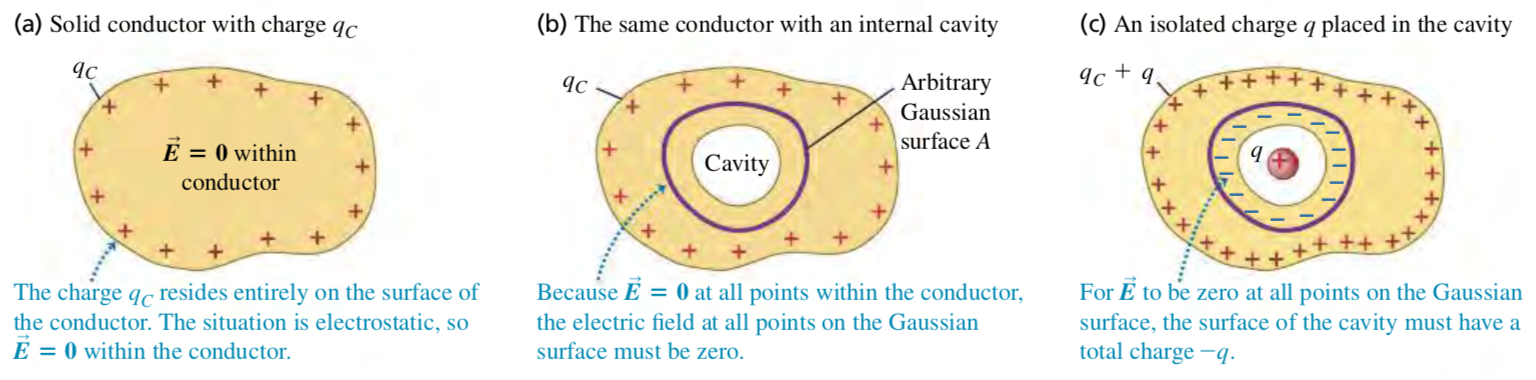
\includegraphics[scale=0.65]{images/electric_fields.png}

\end{itemize}
\end{document}
